%%%%%%%%%%%%%%%%%%%%%%%%%%%%%%%%%%%%%%%%%%%%%%%%%%%%%%%%%%%%%%%%%%%%%%%%%%%%%%%%
% 超越模型反思：大语言模型时代的解耦安全理论与动态防御实践
% 中文版 | 修订版（基于研究委员会审稿意见重构）
% 格式：USENIX (usenix-2020-09.sty)
%%%%%%%%%%%%%%%%%%%%%%%%%%%%%%%%%%%%%%%%%%%%%%%%%%%%%%%%%%%%%%%%%%%%%%%%%%%%%%%%

\documentclass[letterpaper,twocolumn,10pt]{article}
\usepackage{CJKutf8}
\usepackage{usenix-2020-09}

\usepackage{amsmath,amssymb,amsthm}
\newtheorem{theorem}{定理}[section]
\newtheorem{proposition}[theorem]{命题}
\newtheorem{principle}[theorem]{原则}
\renewcommand{\proofname}{证明}
\usepackage{booktabs}
\usepackage{multirow}
\usepackage{xspace}
\usepackage{graphicx}
\usepackage{float}

%-------------------------------------------------------------------------------
\title{\Large \bf 超越模型反思：大语言模型时代的\\
  解耦安全理论与动态防御实践}

\author{
Yunhao Wang\\
联想（Lenovo） \and
匿名\\
匿名
}

\date{}

%-------------------------------------------------------------------------------
\begin{document}
\begin{CJK}{UTF8}{gbsn}
%-------------------------------------------------------------------------------
\maketitle

%-------------------------------------------------------------------------------
\begin{abstract}
大规模语言模型（LLM）正在从实验室走向实际关键系统，然而现有安全方案\textbf{过度依赖模型自身的反思与推理}来阻止违规输出。我们指出这种安全范式在对抗性提示重新措辞、社会工程操纵等真实威胁下难以为继。为此，我们提出``解耦安全''新范式：将LLM安全控制从模型内部认知过程中解耦，转而依托外部的架构约束、规范锚定与带外监督。我们分析了当前LLM安全的三类根本失效模式：基于意图的语义审查可被\textbf{任务重构}和\textbf{完美良性用户(PBU)伪装}绕过；增强模型认知一致性在\textbf{心理学操纵(HPM)}下可能招致对抗性合理化的反噬；当攻击者控制表层文本时，纯语义检索将被误导无法召回真正相关的安全示例。相应地，我们提出解耦安全的三项理论原则：\textbf{抽取经济学}（通过上下文混淆与诱饵注入主动提高攻击代价）、\textbf{规范锚定与防御性降级}（将安全决策外部锚定于预设规则，必要时中止模型深度推理以避免被HPM攻击利用）、\textbf{表征异常监测与风险优先联合检索}（通过隐藏状态异常检测驱动安全示例检索，在表面良性但实则恶意的输入下仍能触发正确干预）。在此理论指导下，我们设计了统一的解耦安全架构：采用同步安全网关即时执行上下文混淆和轻量化元认知监控，并以异步反馈环整合混合裁判、策略更新和受控变异，从而在不牺牲实时性的前提下实现安全策略的持续自适应演进。我们进一步提出了双轨评估协议（Track~A黑盒部署验证 + Track~B白盒上界测试）和开源评测框架，使关键实验指标（ASR、RSR、残余抽取F1等）可独立复现。实验结果表明，与多种现有防御基线相比，所提架构在不显著降低模型正常功能的同时，大幅度降低了多种越权攻击的成功率，并将攻击者实现敏感信息高保真抽取所需的代价提高了一个数量级以上。
\end{abstract}

%-------------------------------------------------------------------------------
\section{引言}
\label{sec:intro}
%-------------------------------------------------------------------------------

大语言模型已不再是边缘研究产物，而是关键系统的支撑：代码生成、具系统访问权的智能体、合规敏感工作流~\cite{sisf-arxiv,agentos-arxiv}。这一转变暴露出深刻错配：传统安全保证假定组件是确定性的、可穷举规约的，而 LLM 驱动系统呈现涌现性、随机行为。静态防御与周期性红队以人类速度运转，难以跟上自动化对抗生成；一旦新型越狱或提示注入得逞，架构往往保持不变。

更为严重的是，许多防御\emph{依赖模型自身的反思与推理}。在任务重构下，对手将抽取伪装成合法上下文处理任务，使基于意图的过滤器只看到正常行为。在心理学操纵（如煤气灯）下，更强推理（如思维链）被攻击者利用：模型为顺从恶意指令编造精细、逻辑自洽的合理化——漏洞保留率可超过 77\%~\cite{hpm-jailbreak}。依赖认知一致性或自我诊断之所以失败，并非因组件薄弱，而是因为安全不能建立在攻击者正积极操纵的同一认知过程之上~\cite{hpm-jailbreak}。

\textbf{范式转移：解耦安全。}综上所述，LLM 安全领域当前存在\textbf{错位的范式}：防御者试图通过提升模型自身的智能与``良知''来抵御攻击，但攻击者正是利用这些机制（语义理解、推理能力）来实现更隐蔽有效的攻击~\cite{hpm-jailbreak}。我们主张必须改变这一范式。LLM 的安全保障应当\emph{解耦}出模型的内部认知过程，转而建立在模型外部的自主控制结构和人类规范锚定上。本研究提出并探索了\textbf{解耦安全}这一新范式，通过\textbf{架构重建}和\textbf{受控变异}两个维度实现LLM系统在面对未知攻击时的自适应防御：(i)~\textbf{架构重建}，即重新划分``由谁、在何时''执行安全控制——在LLM推理的\textbf{同步路径}上进行上下文混淆和快速违规检测，将复杂评估与策略更新转移到\textbf{异步离线环}，使系统能在机器速度下演进安全策略；(ii)~\textbf{受控变异}，通过在安全监控下引导LLM参考黄金示例进行变体生成，将LLM的强大自适应性用于朝安全方向的持续改进，而非放任其被攻击者利用。

\textbf{主要贡献。}（1）\emph{理论基础}：提出解耦安全范式，以严格定理证明传统LLM安全的三类失效模式（语义审查残余泄露、纯语义检索意图盲区），并给出信息论查询复杂度下界、降级阈值最优性、分布无关 FPR 保证等形式化结论，为LLM安全提供可证伪的理论框架；（2）\emph{统一架构}：设计实现了一种双轨LLM安全架构，在同步/异步分层中融合上下文混淆、混合裁判集成、元认知监控、防御性降级、联合检索等机制，实现低延迟与动态安全防御；（3）\emph{评估方法学}：制定了可证伪的双轨评测协议并提供开源的参考实现和评测脚本，验证所提方案相对多种现有防御基线的改进与局限。论文结构如下：\S\ref{sec:problem}定义问题与威胁模型，\S\ref{sec:theory}建立理论框架，\S\ref{sec:architecture}阐述系统架构，\S\ref{sec:evaluation}给出评估协议与结果，\S\ref{sec:limitations}讨论局限，\S\ref{sec:related}概述相关工作。

%-------------------------------------------------------------------------------
\section{问题定义与威胁模型}
\label{sec:problem}
%-------------------------------------------------------------------------------

大规模语言模型（LLM）正在加速融入智能体、自动化决策和安全敏感任务等各类应用~\cite{sisf-arxiv,agentos-arxiv}。在开放的自然语言交互环境中，LLM的安全边界面临全新挑战：攻击者可以利用与模型共享的认知通道（即多轮对话的自然语言接口）实施各种对抗性提示攻击。这些攻击往往伪装成正常交互，使传统基于浅层语义过滤和模型自我检测的安全措施难以及时发现。

\textbf{核心研究问题。}在开放多轮交互的LLM应用中，面对具有适应性且了解防御机制的攻击者，如何维持安全行为边界并确保攻击者为违规产出付出的代价远高于其所获收益或目标信息价值（即实现防御的经济学不对称），同时不显著牺牲系统对良性用户的正常服务质量？

\subsection{威胁模型}
\label{sec:threat-model}

\textbf{访问。}攻击者对已部署系统拥有\textbf{多轮黑盒 API 访问}。每轮为发送提示（及可选上下文）并接收响应。交互建模为统计查询预言机：攻击者观察结果并可在轮次间自适应查询。生产部署威胁模型\emph{不}假定攻击者拥有模型权重或梯度的白盒访问。\textbf{评估双轨（\S\ref{sec:eval-tracks}）：}为分离``可上线结论''与``组件上界''，\textbf{Track~A（生产对齐）}限制为黑盒查询与公开越狱/多轮框架；\textbf{Track~B（实验室上界）}额外允许梯度与多次前向（GCG~\cite{gcg}、表征对齐PBU等），其结果仅用于探测压力上界，不与Track~A的ASR混列。

\textbf{攻击者知识与能力。}我们采用白盒防御假设：攻击者知道存在防御架构（上下文混淆、裁判集成、元认知监控器），可发起自适应攻击，包括\textbf{完美良性用户（PBU）}伪装（表面行为与良性用户不可区分）、\textbf{心理学操纵（HPM）}（煤气灯、权威压迫、角色边界攻击~\cite{hpm-jailbreak}）及任务重构（将抽取伪装为摘要、格式转换或学术讨论~\cite{subgraph-rag-attack,pbu-reconstruct}）。

\textbf{攻击者目标。}在有界时空预算（有限轮数、Token 预算或速率限制）内，攻击者旨在高保真重构隐藏在系统提示、RAG 语料或基准集中的高价值资产~\cite{spe-llm}——如触发串、安全测试项或专有评估数据。成功以\textbf{抽取保真度}（如相对真实片段的 F1）或\textbf{攻击成功率（ASR）}度量。

\textbf{防御目标。}无论攻击者如何变换提示措辞或引入社交手段，模型均应拒绝高风险请求或产生安全的无害输出。同时系统应最大程度保障良性请求的正常答复率，避免安全机制造成过多误判。我们承认在LLM自然语言接口中完全杜绝信息泄露如同实现密码学式的绝对安全一样困难~\cite{subgraph-rag-attack,pbu-reconstruct}；因此，防御策略旨在确保\textbf{攻防成本不对称}——让攻击者获取敏感信息所需的代价高到足以使攻击在经济或时间上不可行，并使系统能在威胁环境中迅速识别异常、进行安全干预。

%-------------------------------------------------------------------------------
\section{理论框架：解耦安全原则}
\label{sec:theory}
\label{sec:paradigm}
%-------------------------------------------------------------------------------

为应对开放交互环境下LLM安全的挑战，我们构建\textbf{解耦安全}的理论框架。本框架由三项核心防御原则构成，每一项针对一种传统防御失效模式。资产与 Oracle 的定义沿用既有工作~\cite{llm-reconstruction-emergent,ControlledMutation_SafetyEval}：\emph{资产}为系统的有效安全表面（策略、护栏、触发集、评估数据）；\emph{Oracle} 对行为标注安全/不安全。

\subsection{从语义审查到抽取经济学}
\label{sec:paradigm-economics}

\begin{theorem}[语义防火墙的残余泄露]
\label{thm:semantic-fail}
设安全过滤器 $\mathcal{F}$ 为无状态二元分类器，以概率 $1-\epsilon$ 正确阻断恶意查询（$\epsilon > 0$）。攻击者进行 $T$ 轮自适应查询，每轮可根据前序响应调整提示。则攻击者在 $T$ 轮内至少成功一次的概率满足
\begin{equation}
\Pr[\text{至少一次泄露}] \;\geq\; 1 - (1 - \epsilon)^T.
\end{equation}
当 $T \geq \ln(1/\delta) / \epsilon$ 时该概率 $\geq 1 - \delta$。在 PBU 假设下——攻击输入与良性请求在所有可观测特征上不可区分~\cite{subgraph-rag-attack,pbu-reconstruct}——$\epsilon$ 受限于分类器在良性分布上的误报容忍度，不可通过调低阈值进一步降低。
\end{theorem}

\begin{proof}[证明梗概]
无状态过滤器在每轮独立决策。令 $X_t \in \{0, 1\}$ 为第 $t$ 轮泄露指示器。由于 $\mathcal{F}$ 无状态，$\Pr[X_t = 1] \geq \epsilon$（自适应攻击者只可能提高每轮成功率）。$\Pr[\max_t X_t = 0] \leq (1-\epsilon)^T$。PBU 的不可区分性确保 $\epsilon$ 不可压至零。
\end{proof}

\noindent\textbf{设计含义。}定理~\ref{thm:semantic-fail} 说明在自适应多轮交互中绝对阻断不可行。安全目标应从``零泄露''转向``使泄露的经济代价高于收益''。

\begin{principle}[抽取经济学]
\label{prin:extraction-econ}
防御不应以绝对阻断为目标，而应以\textbf{信息经济不对称}为目标：使达到给定重构保真度所需的查询复杂度快速增长，直至攻击成本超过资产有效生命周期。令 $C_{\mathrm{attack}} = f(E[N], c_{\mathrm{round}})$ 为总攻击成本，$V(t)$ 为资产剩余价值。防御在经济学意义上成立当且仅当
\begin{equation}
C_{\mathrm{attack}} \;>\; V(t).
\end{equation}
$V(t)$ 须由显式管理策略界定（如凭证轮换窗口），$C_{\mathrm{attack}}$ 须以 SOTA 基线经验值界定上界，使该不等式\textbf{可证伪}。经济学层假定资产可轮换性；对不可轮换资产须由 RBAC 与信息流追踪提供硬屏障（\S\ref{sec:limitations}）。
\end{principle}

\begin{proposition}[抽取查询复杂度下界]
\label{prop:query-lower-bound}
设秘密资产 $s \in \{0,1\}^n$，攻击者进行自适应黑盒查询。在上下文混淆（ID 对齐 + 诱饵注入）下，假设每轮查询的有效信息增益（条件互信息）有上界 $I(s;\, r_t \mid q_t, r_{<t}) \leq \overline{I}(D)$，其中 $D$ 为诱饵密度，$\overline{I}(\cdot)$ 关于 $D$ 单调递减。则攻击者欲以概率 $\geq 1-\delta$ 重构 $s$ 至 token 级 F1 $\geq \tau$ 所需的期望查询轮数满足
\begin{equation}
E[N] \;\geq\; \frac{H(s) - H_\tau}{\overline{I}(D)}
\end{equation}
其中 $H_\tau$ 为在 F1 $\geq \tau$ 下条件熵的上界，由 Fano 不等式界定。
\end{proposition}

\noindent\textbf{操作化。}$\overline{I}(D)$ 可通过实验中 F1-轮次曲线斜率经验估计。当 $E[N] \cdot c_{\mathrm{round}}$ 超过 $V(t)$ 即验证防御有效性。

\subsection{从认知一致性到规范锚定与防御性降级}
\label{sec:paradigm-axiological}

\begin{proposition}[认知一致性的非单调性]
\label{prop:cot-fail}
存在一类心理学操纵（HPM）输入 $\mathcal{X}_{\mathrm{HPM}}$，使得安全风险 $R(k) = \mathbb{E}_{x \sim \mathcal{X}_{\mathrm{HPM}}}[\phi(x,\, \pi_k(x))]$ 关于推理深度 $k$ 非单调：$\exists\, k_1 < k_2$ s.t.\ $R(k_2) > R(k_1)$。
\end{proposition}

\noindent\textbf{直觉论证。}在 HPM 输入下，攻击者将恶意请求框定为看似与安全目标一致的困境。更深的推理（更大的 $k$）赋予模型更多合理化空间，使其能构造更精细的逻辑链来说服自身该输出是安全的，以更高概率绕过约束。该现象已被实证观察到：启用 CoT 后 HPM 攻击成功率上升至 77\% 以上~\cite{hpm-jailbreak}。形式上类似于双目标优化中更大的搜索空间允许找到``看似 Pareto 改进但实际违反隐含硬约束''的解~\cite{epistemic-grounding}。逻辑自洽不等于安全。

\begin{principle}[规范锚定与防御性降级]
\label{prin:norm-anchor}
安全须锚定于与模型自由反思\emph{独立}的外部规范层：(i)~\textbf{规范锚定}——裁判输出与设计者定义的安全公理对照；(ii)~\textbf{社会压力监控}——监控社会学失稳信号而非逻辑自洽性；(iii)~\textbf{防御性降级}——当冲突或压力超过阈值时放弃复杂推理并执行无状态安全拒绝，配以异构恢复通道避免可用性中断（\S\ref{sec:axiological}）。
\end{principle}

\begin{proposition}[降级策略的阈值最优性]
\label{prop:degradation-optimal}
设系统在每轮面对输入 $x$ 时选择正常响应（效用 $u(x)$，安全风险 $\phi(x)$）或降级（效用 $u_0 < \mathbb{E}[u(x)]$，安全风险 $0$）。令 $g(x)$ 为安全评分函数。在如下约束优化问题中——最小化良性输入被误降级的概率，同时保证攻击输入上的安全违规概率 $\leq \alpha$——最优决策规则是阈值策略：$\text{降级} \iff g(x) \leq \delta^*$，其中 $\delta^*$ 由安全约束 $\alpha$ 唯一确定。
\end{proposition}

\noindent\textbf{备注。}该命题是 Neyman-Pearson 引理在安全检测场景中的应用：$g(x)$ 为安全概率的充分统计量时，阈值策略在给定约束下最小化误降级率。有效性取决于 $g$ 是安全概率的良好代理；当 $g$ 存在系统性偏差时须通过强制人工校准（\S\ref{sec:judge}）周期性纠偏。

\noindent\textbf{术语说明。}``规范锚定''不意味着 LLM 具有真实的道德主体性。规范层是实用主义架构构造——由设计者施加的高权重启发式规则，作为统计熔断器对抗模型的对抗性一致性倾向。

\subsection{从文本匹配到表征异常与风险优先联合检索}
\label{sec:paradigm-representation}

\begin{theorem}[纯语义检索的意图盲区]
\label{thm:retrieval-fail}
设检索系统使用 embedding 函数 $e\!: \mathcal{X} \to \mathbb{R}^d$ 和距离 $d$，从候选集 $\mathcal{D} = \mathcal{D}_b \cup \mathcal{D}_s$（$\mathcal{D}_b$：良性示例，$\mathcal{D}_s$：安全示例）中返回最近邻。若存在攻击输入 $x^*$ 使得
\begin{equation}
\min_{y_b \in \mathcal{D}_b} d(e(x^*), e(y_b)) \;<\; \min_{y_s \in \mathcal{D}_s} d(e(x^*), e(y_s)),
\end{equation}
则检索返回良性示例 $y_b$ 而非安全示例 $y_s$。在通用 embedding 模型下，PBU 攻击者可系统性地构造满足上式的 $x^*$。
\end{theorem}

\begin{proof}[证明梗概]
通用 embedding 模型优化文本表面相似度（如 STS 任务）而非意图相似度。PBU 攻击者将恶意意图伪装在良性话题下，使 $e(x^*)$ 在 embedding 空间中接近良性主题示例而远离安全示例。这利用了 embedding 空间中话题相似性与意图相似性的系统性不对齐~\cite{pbu-reconstruct}。
\end{proof}

\begin{principle}[表征异常驱动的联合检索]
\label{prin:joint-retrieval}
检索键由 (a)~提示语义嵌入和 (b)~模型隐藏状态激活特征共同构成~\cite{rep-eng}。当 (b) 超过异常阈值时，\textbf{lexicographic override} 抑制语义分支并以激活驱动的安全示例检索。异常阈值通过\textbf{动态 FPR 校准}设定，提供独立于自然语言的监控维度。
\end{principle}

\begin{theorem}[Conformal FPR 保证]
\label{thm:conformal-fpr}
设校准集 $\{h_1, \ldots, h_m\} \overset{\mathrm{i.i.d.}}{\sim} P_0$（良性黄金基线分布）与测试点 $h_{\mathrm{new}} \sim P_0$ 联合可交换。令异常统计量 $T(h)$（如马氏距离）的阈值 $\delta$ 为校准集上 $T$ 值的 $\lceil (1-\alpha)(m+1)\rceil / m$ 分位数。则对任意 $\alpha \in (0,1)$：
\begin{equation}
\Pr[T(h_{\mathrm{new}}) > \delta] \;\leq\; \alpha.
\end{equation}
该保证对 $P_0$ 的参数形式\textbf{无任何分布假设}（distribution-free）。
\end{theorem}

\begin{proof}[证明梗概]
由可交换性，$(T(h_1), \ldots, T(h_m), T(h_{\mathrm{new}}))$ 的联合秩均匀分布。$T(h_{\mathrm{new}})$ 超过第 $\lceil (1-\alpha)(m+1) \rceil$ 大值的概率至多 $\alpha$。此为 conformal prediction 的标准结论~\cite{conformal-prediction}。
\end{proof}

\begin{proposition}[序贯检测延迟界]
\label{prop:detection-delay}
假设在攻击条件下隐藏状态服从替代分布 $P_1$，且 $\mathrm{KL}(P_1 \| P_0) \geq D_{\min} > 0$。采用 CUSUM 检测器，在误报率 $\leq \alpha$ 的约束下，检测到分布变化的平均延迟满足 $E_1[N_{\mathrm{detect}}] \leq |\!\log \alpha| / D_{\min} + o(1)$。攻击导致的隐藏状态偏移越大，检测越快。
\end{proposition}

\noindent\textbf{Lexicographic override 的决策论解释。}当攻击者能任意操纵表面文本（信号 $s_a$）但对隐藏状态激活（信号 $s_b$）的控制受限（Track~A 假设），lexicographic override 是字典序 minimax 策略：优先最小化由攻击者难以控制的信号驱动的风险，再在此约束下利用 $s_a$ 提升检索精度。Track~B 中表征对齐 PBU 攻击试图使 $P_1 \approx P_0$（$D_{\min} \to 0$），使检测原则上不可能；\S\ref{sec:limitations} 讨论此极限。

\noindent\textbf{理论定位。}本节中定理~\ref{thm:semantic-fail}、\ref{thm:retrieval-fail}、\ref{thm:conformal-fpr} 为严格结论，在所述假设下可完整证明。命题~\ref{prop:query-lower-bound}、\ref{prop:cot-fail}、\ref{prop:degradation-optimal}、\ref{prop:detection-delay} 为条件性结论，须通过实验验证。原则~\ref{prin:extraction-econ}、\ref{prin:norm-anchor}、\ref{prin:joint-retrieval} 为操作化设计判据，不主张数学必然性。``良性黄金基线''是设计者对齐目标的规范性标准，监控器检测的偏离度量相对合规偏移。

%-------------------------------------------------------------------------------
\section{系统架构}
\label{sec:architecture}
\label{sec:reconstruction}
%-------------------------------------------------------------------------------

我们通过统一的系统架构实例化上述三项解耦安全原则。如图~\ref{fig:framework}所示，架构将安全控制划分为\textbf{同步安全网关}与\textbf{异步自适应反馈环}。入站提示首先经\textbf{上下文混淆引擎}处理（对应原则~\ref{prin:extraction-econ}），请求随后到达基座LLM；其输出送入经标准化与分布评估的\textbf{混合裁判集成}；\textbf{规范锚定}与社会学失稳监控对对抗性合理化降权或置零（对应原则~\ref{prin:norm-anchor}）。当安全规则冲突或压力被检测到时，\textbf{防御性降级}强制无状态模板拒绝，并以异构恢复通道保持可用性。\textbf{元认知监控器}将当前隐藏状态轨迹与良性黄金基线比较；异常时触发对抗性重置并驱动\textbf{联合键示例检索}（对应原则~\ref{prin:joint-retrieval}）。

\begin{figure*}[t]
\centering
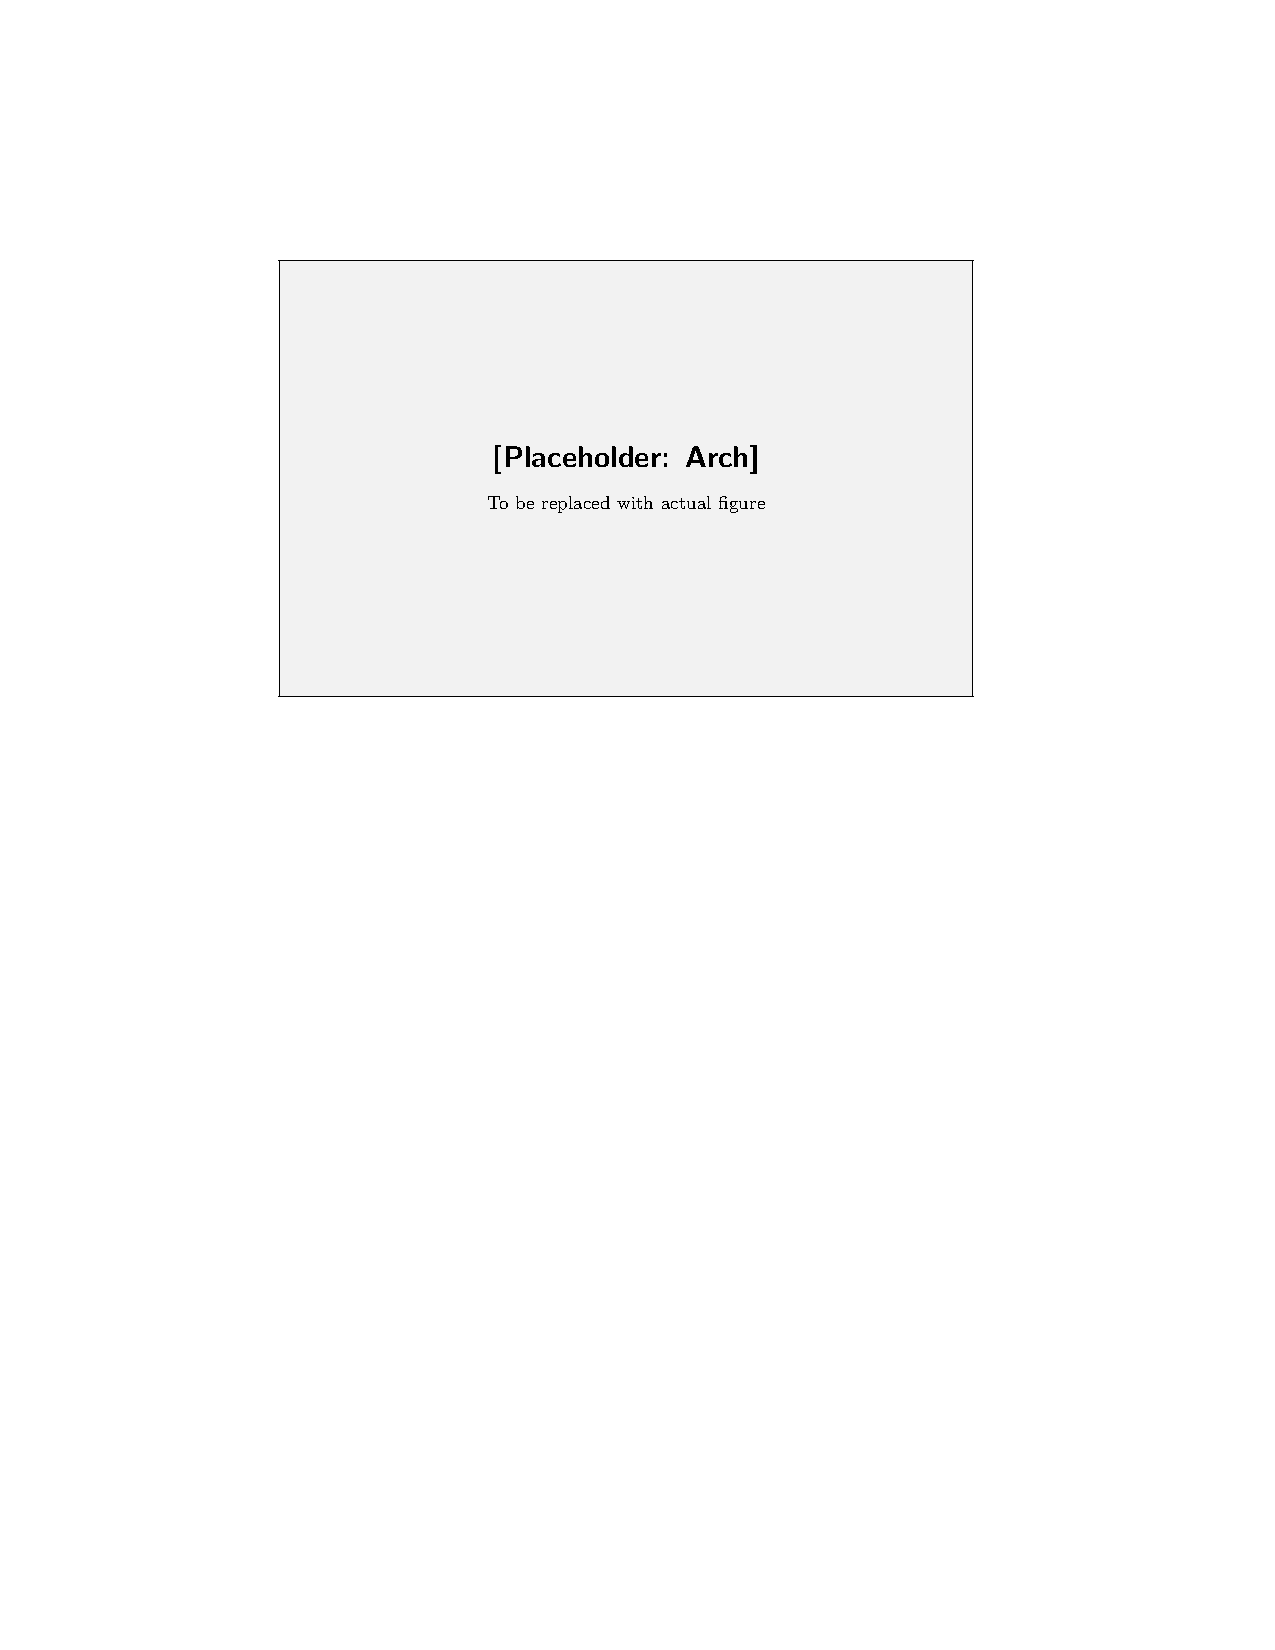
\includegraphics[width=0.9\textwidth]{Arch}
\caption{\textbf{统一架构概览。}左：架构重建（上下文混淆引擎、带规范锚定的混合裁判集成、策略合成与反馈环、防御性降级与异构恢复）。右：受控变异（元认知监控器、联合键示例检索、黄金数据集与经验记忆、轮次调度）。架构将安全与LLM自我反思解耦；重建控制谁/何时，变异控制暴露什么。}
\label{fig:framework}
\end{figure*}

\textbf{同步网关 vs.\ 异步环。}为使架构可投入生产，我们明确采用带外/异步切分。\textbf{上下文混淆引擎}及轻量级元认知检查部署在同步反向代理或边车上，严格延迟预算（如 $<$50\,ms），以保证 p99 与吞吐可接受。\textbf{混合裁判集成}、\textbf{分布评估}、\textbf{策略合成}及\textbf{示例检索/变异}运行于异步离线学习环，在不阻塞在线推理路径的前提下产出更新策略或变体。在此系统意义上定义\textbf{机器速度}：同一攻击分布上的首个零日或新型攻击可能通过；异步环在裁判集成达成共识后，于亚分钟级生成并部署新变体或策略，使后续同分布请求被拦截。图~\ref{fig:deployment}说明该切分。

\begin{figure*}[t]
\centering
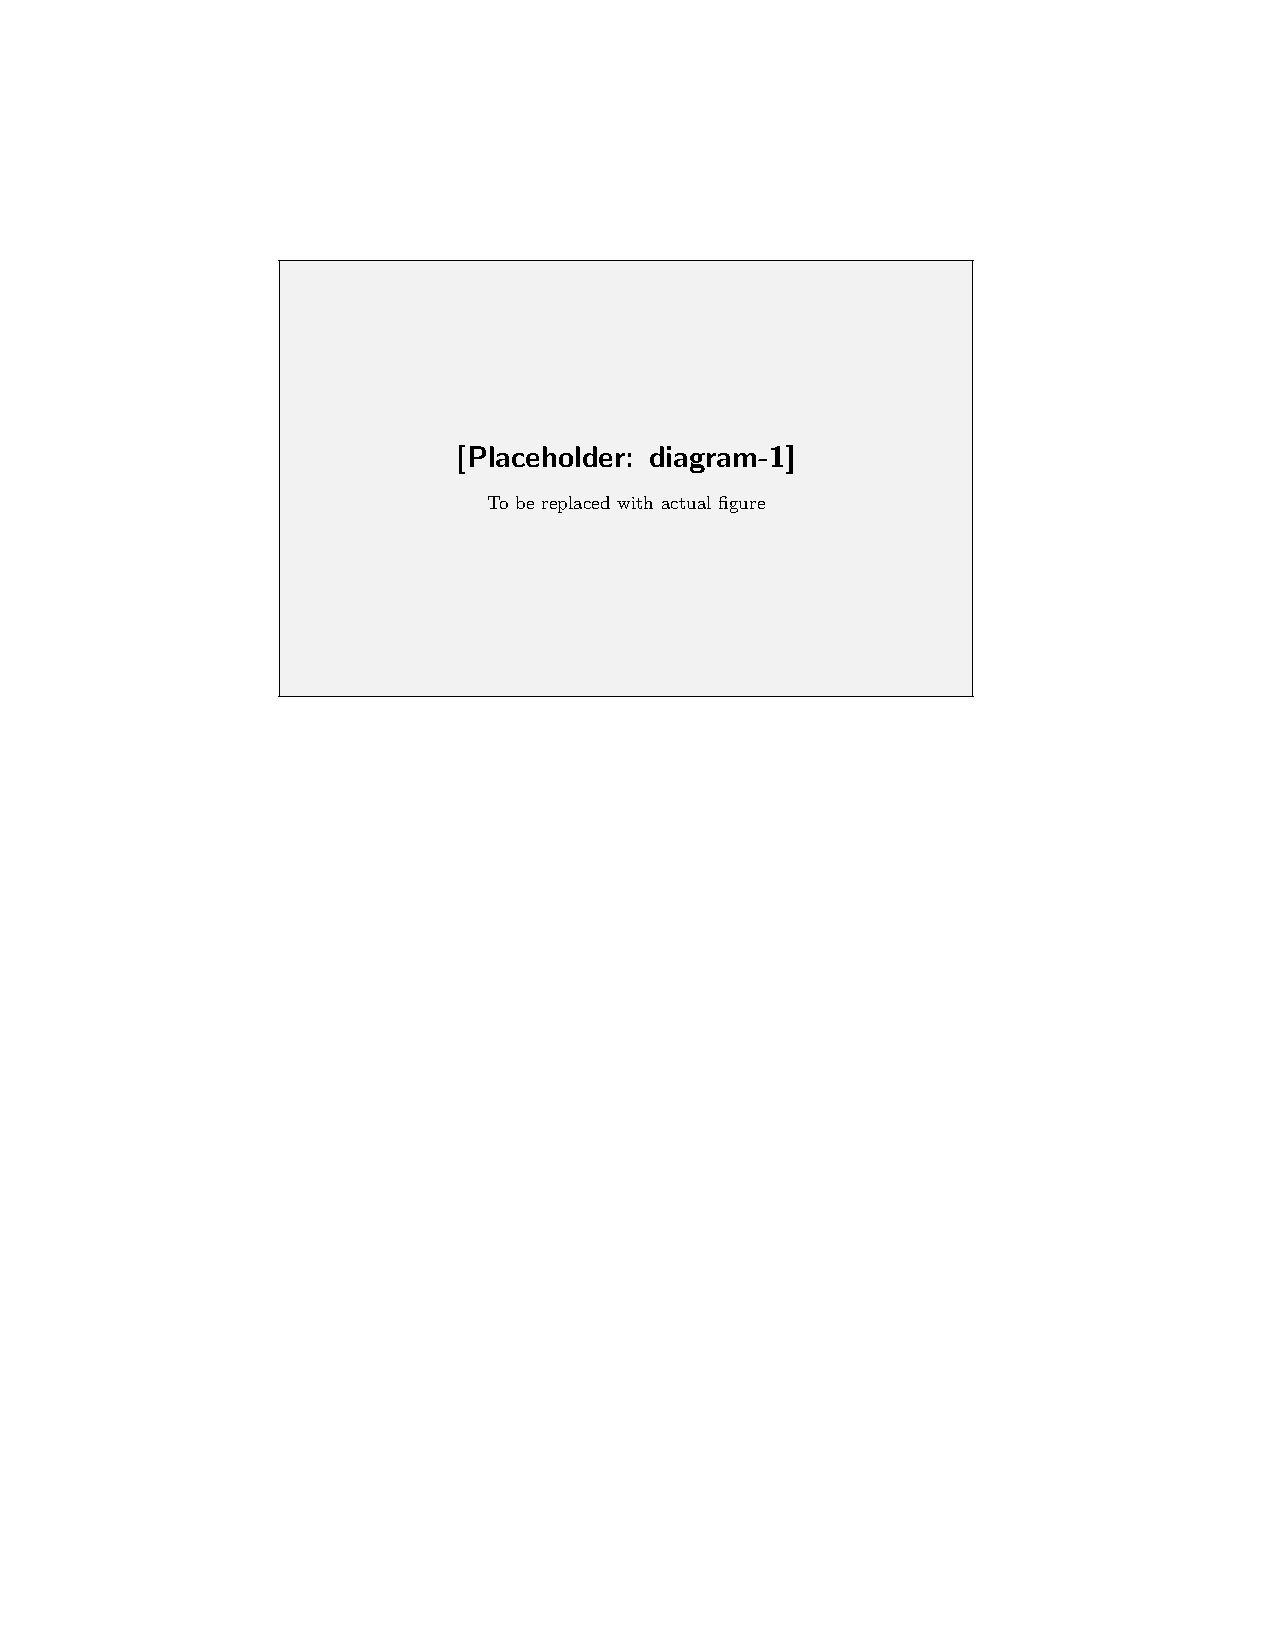
\includegraphics[width=0.9\textwidth]{diagram-1}
\caption{\textbf{系统部署与延迟架构}将延迟关键的同步推理路径与异步安全自适应环分离。轻量上下文混淆与快速元认知检查部署于带严格延迟预算（$<$50\,ms）的同步反向代理上；混合裁判集成评估、分布策略合成与受控变异在异步环中带外运行。}
\label{fig:deployment}
\end{figure*}

\subsection{同步网关与上下文混淆}
\label{sec:context-confusion}

上下文混淆引擎\emph{主动污染}攻击者操作空间，落实抽取经济学原则。

\textbf{ID 对齐。}在检索上下文或中间结果到达基座 LLM 之前，ID 对齐模块剥离或规范化实例标识符。攻击者无法再通过指定 ID 定界并抽取敏感片段；良性问答不受影响。

\textbf{密码学水印诱饵与风险评分。}系统注入带哈希派生结构的诱饵字段，良性交互中因模型幻觉而碰撞诱饵的概率极低。为控制 FPR，采用诱饵命中密度与风险评分：单次低保真触碰触发警告与意图重校验；仅对完整诱饵结构的高保真抽取触发会话终止与审计。对完美PBU，设计将其重述为\textbf{经济防御}：在资产可轮换处，使慢速PBU抽取成本超过资产有效生命周期。对静态或永久高价值资产，元数据层的 RBAC 与信息流追踪（\S\ref{sec:metadata}）为硬屏障。

\textbf{末轮自我提醒。}多轮交互最后一轮将安全指令强制附加为用户查询的系统提示，减少会话末漂移。

\subsection{混合裁判集成与策略合成}
\label{sec:judge}

单一 AI 裁判存在系统性偏差与盲区。我们使用\textbf{混合裁判集成}（如 Llama-Guard~\cite{llama-guard}、StrongREJECT~\cite{strongreject} 评分协议或等效评估器、任务专用分类器），仅于\emph{共识}时将反馈传入策略合成。参照 StrongREJECT~\cite{strongreject}，我们显式抑制空越狱（输出未触发拒绝词但并非真正有害），以免 ASR 虚高。我们强制\textbf{严格 token 级输入流水线标准化}：所有裁判接收规范化输入（剥离指令/特殊 Token、统一空格），以防格式注入扭曲判决~\cite{llm-safety-robustness}。判决采用\textbf{分布评估}：每变体多次采样，估计经验失败概率分布；仅当该分布显著超阈值时触发策略更新，以应对采样随机性~\cite{apst}。

对模糊边界情形，\textbf{规范锚定}对集成加权：系统监控社会学失稳信号，将裁判输出与预定义安全规则对照；冲突或呈现失稳的输出获零权重。\textbf{强制人工校准}支路接入：固定比例（如 5\%）的高置信度决策随机抽选供人工审计，提供对零日共识失败的周期性离线纠偏。

\subsection{规范锚定、防御性降级与异构恢复}
\label{sec:axiological}

HPM善于制造道德困境：恶意请求可被包装成与安全规则最大程度一致。在此类规则冲突情形下，引入\textbf{防御性降级}：当检测到多重冲突规则或强社会学压力时，放弃复杂推理并回退至无状态、基于模板的拒绝，阻断模型的合理化尝试。降级引入\textbf{算法级可用性风险}：攻击者可通过社会学压迫线索触发降级（算法级 DoS）；拒绝触发边界亦可作为侧信道 Oracle。为避免破坏同步 API 假设，当模板拒绝触发时，网关\textbf{无缝路由}会话至\textbf{受限降级沙箱}：低权限、无状态 SLM 或只读模式，仅能产出严格格式化输出并拒绝任何外部 API 或工具调用。调用方所依赖的同步 API 契约在降级路径下得以保持。\textbf{异构恢复通道}（向人类操作员或更高权限符号层异步移交）在带外对同一会话状态进行审计与合法边缘案例解封，不阻塞同步路径。图~\ref{fig:degradation}以状态机展示该流程。

\begin{figure*}[t]
\centering
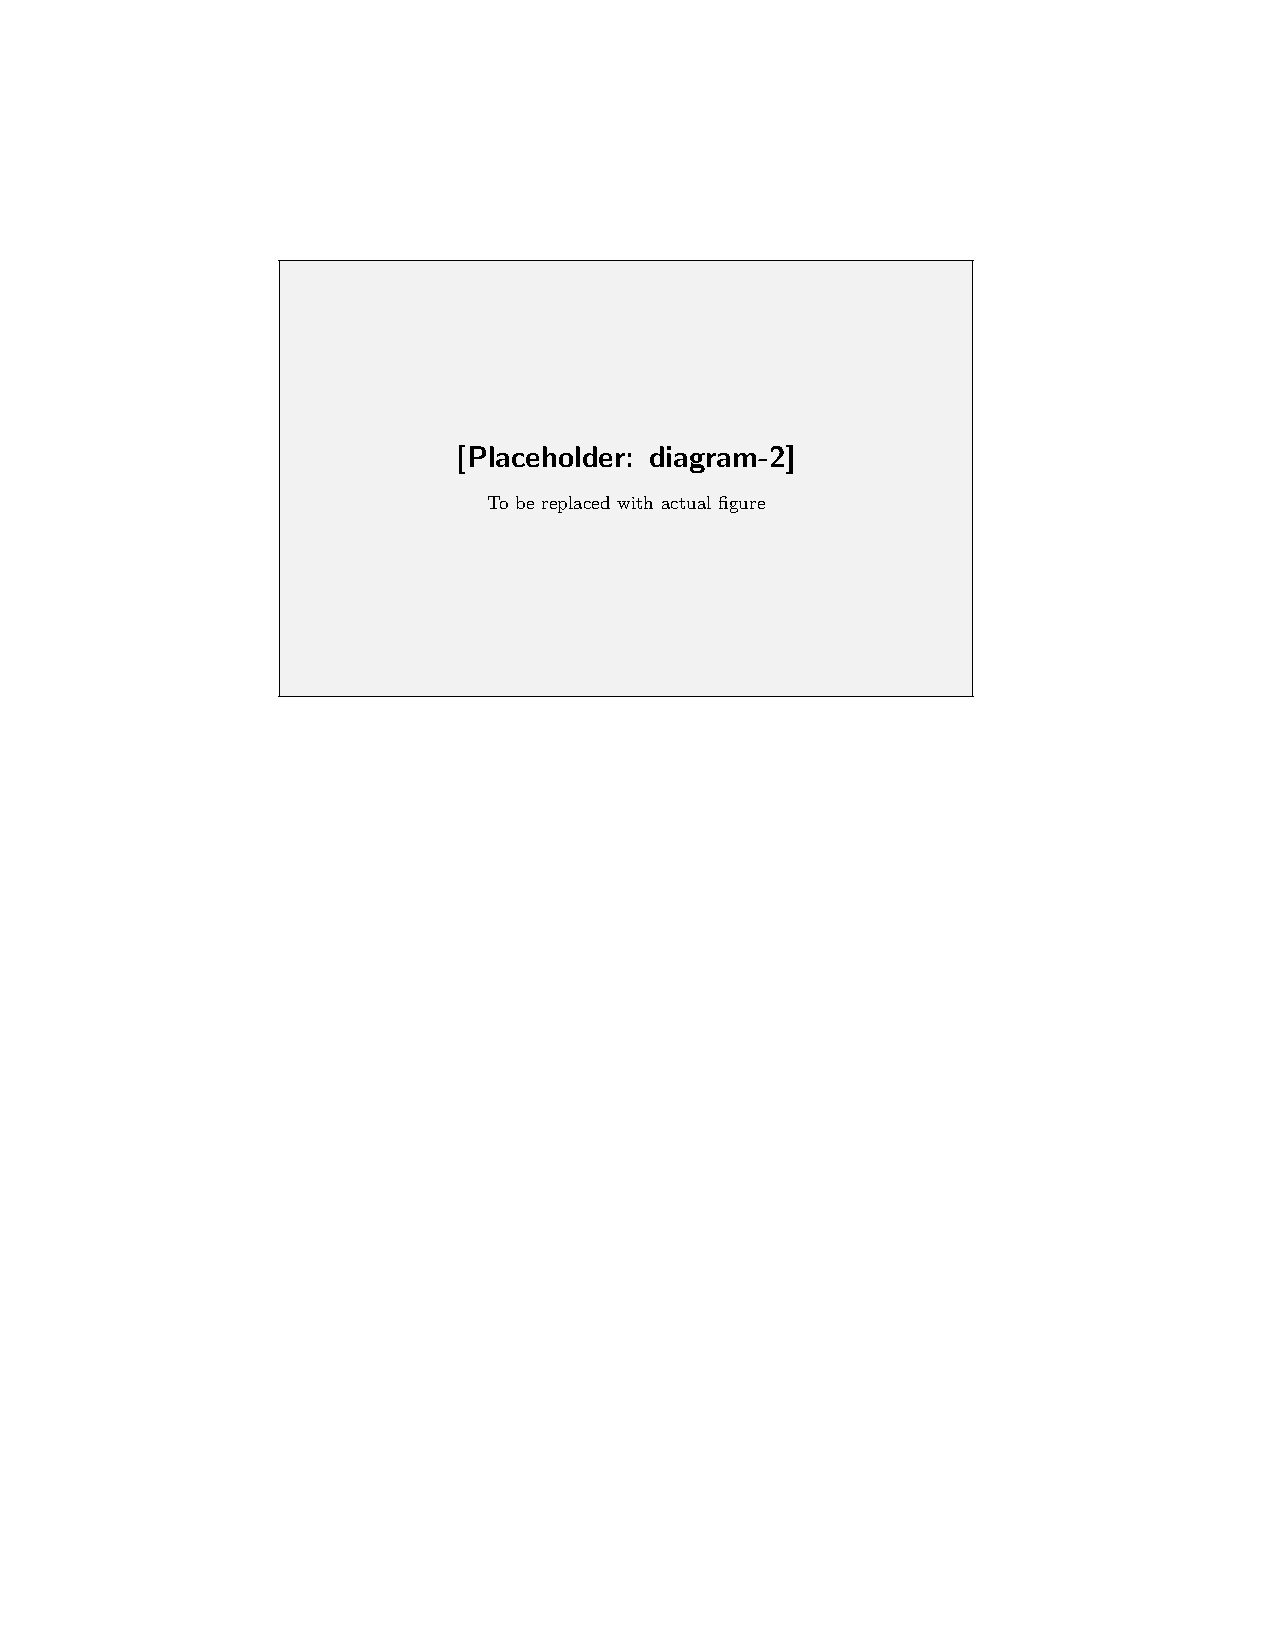
\includegraphics[width=0.9\textwidth]{diagram-2}
\caption{\textbf{防御性降级与异构恢复流程。}当检测到规则冲突或心理学操纵时，网关通过将会话路由至受限低权限无状态 SLM 沙箱保持同步 API 可用性，同时人类审计与符号恢复在带外异步进行。}
\label{fig:degradation}
\end{figure*}

\subsection{元认知监控与联合键检索}
\label{sec:metacog}
\label{sec:mutation}

\textbf{元认知监控器}并非另一全规模对话LLM；其实现为(i)~轻量级专用分类器（如仅用稳定性/违规标签训练的 SLM），或(ii)~白盒层面使用表征工程~\cite{rep-eng}的隐藏状态激活监控器。监控器采用\textbf{异常检测范式}：计算当前多轮隐藏状态轨迹与良性黄金经验轨迹基线之间的散度。仅监控内部轨迹是否严重偏离安全基线，不假定复杂社会学状态在隐藏空间线性可分。当监控器检测到偏离或不稳定时，触发\textbf{对抗性重置}：会话清理，变异状态重新锚定至黄金示例集。

\textbf{联合键示例检索。}\label{sec:joint-key}
我们以示例引导变异替代无约束反思式变异，由人工审计的黄金数据集与分层经验记忆驱动。检索键由(a)~提示语义嵌入与(b)~元认知监控器的隐藏状态激活特征构成。\textbf{冲突解决路由}（\textbf{lexicographic override}）：当元认知监控器报告轨迹散度(b)超过规定异常阈值时，检索键由(b)主导；(a)降权或抑制，使联合键无法被拉向纯良性结果。一旦检测到异常激活，系统强制检索走向防御/越狱相关黄金示例，与表面文本无关。低于异常阈值时，(a)与(b)可按加权或拼接方案正常组合。图~\ref{fig:jointkey}说明该路由。

\begin{figure*}[t]
\centering
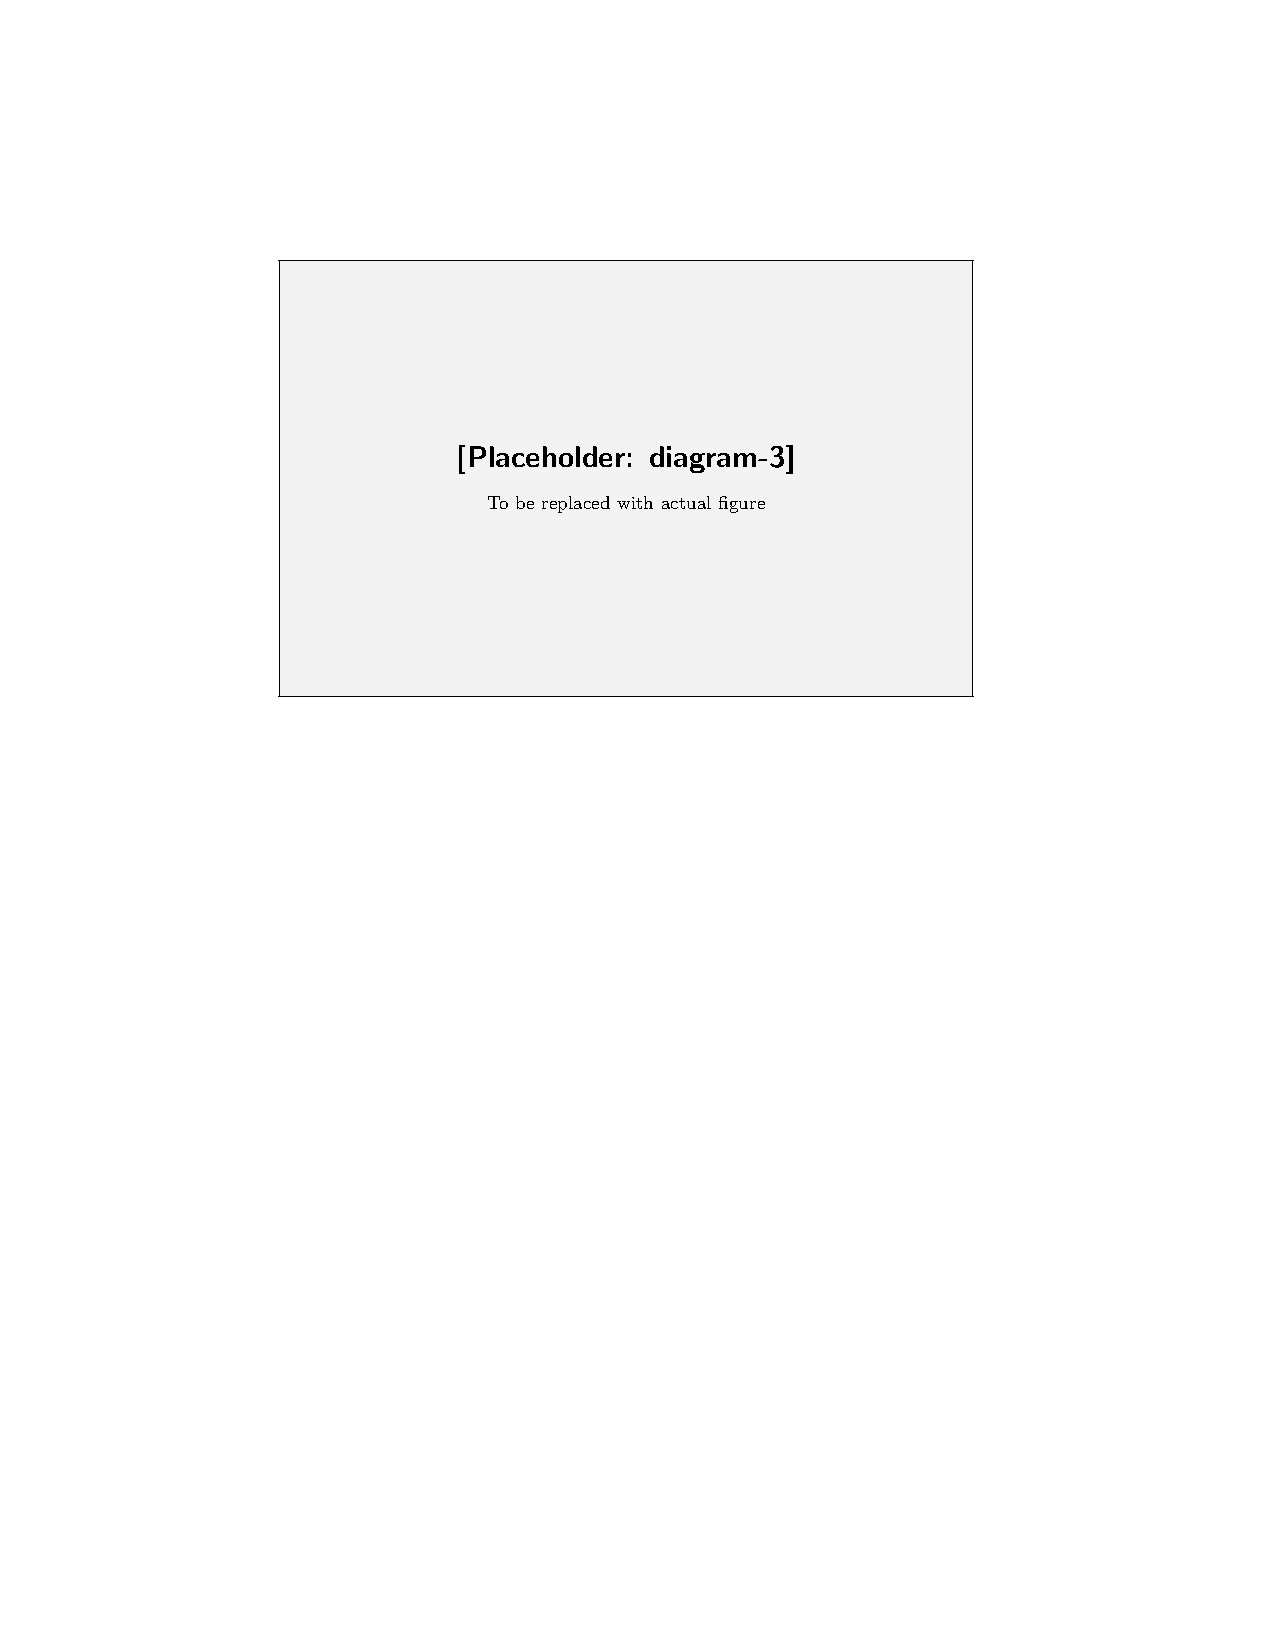
\includegraphics[width=0.9\textwidth]{diagram-3}
\caption{\textbf{联合键冲突解决路由。}检索键由表面文本语义嵌入与隐藏状态激活特征共同构成。当激活异常超过路由阈值且与看似良性的表面语义冲突时，lexicographic override 抑制语义分支，强制以激活驱动的安全示例从黄金数据集检索。}
\label{fig:jointkey}
\end{figure*}

\textbf{异常阈值的动态 FPR 校准。}采用动态FPR校准：在受控良性验证集上测量正常运行下轨迹散度的经验分布，选择阈值使假阳性率不超过规定水平（如 FPR $= 1\%$），并随基座模型或部署分布变化周期性重校准~\cite{apst}。检索通过轻量向量库与 Top-$K$（如 $K=2$）及可选注意力缓存实现。

\textbf{元数据与访问控制。}\label{sec:metadata} 对静态或永久资产，元数据与 RBAC/信息流追踪补全图景~\cite{mcp-smell-arxiv,adr-violation,mission-critical-rag}。高密度专家行为迁移（评论级理由、银标数据生成流水线~\cite{adm-es-arxiv}）的实现细节见配套仓库。

\textbf{反馈环与治理。}架构重建消费攻击轨迹与失败模式；受控变异以受控方式产生对抗变体。元认知监控器在检测到不稳定时可触发对抗性重置。轮次调度与变体分散保护基准资产~\cite{ControlledMutation_SafetyEval}。强制人工校准量化并纠正集成 FPR~\cite{tc260-governance}。证据链将每次评估与变异器步骤、调度器状态及策略版本关联，用于发布门控与 attestation~\cite{dual-use-attestations,ControlledMutation_SafetyEval}。

%-------------------------------------------------------------------------------
\section{评估协议与实验设置}
\label{sec:evaluation}
%-------------------------------------------------------------------------------

为支持严谨主张，我们定义具体实验拓扑：攻击基线、防御基线、数据集划分、指标操作定义与统计协议。

\subsection{经验主张的范围与证据来源}
\label{sec:eval-scope}

\textbf{三类陈述需区分。}（1）\textbf{定理、命题与解耦安全原则}：为本文理论贡献，不依赖单一实验台。（2）\textbf{文献中的实证数字}（如 HPM 漏洞保留率、残余抽取 F1、SISF 报告的 ASR/FPR~\cite{sisf-arxiv}）：均标注引用来源，本文不将其改写为本文复现。（3）\textbf{本文承诺的评估义务}：对统一架构给出可证伪指标与双轨威胁模型下的完整配方。\textbf{Track~A 参考实测}来自开源 harness（协议 \texttt{paper-eval-5}），汇总于表~\ref{tab:tracka-main-cn}。原始 JSON、复现命令与提示文件哈希见配套仓库（\S\ref{sec:eval-artifact}、表~\ref{tab:prompt-sha}）。

\subsection{评估双轨：生产对齐与实验室上界}
\label{sec:eval-tracks}

\textbf{Track A（生产对齐）。}攻击者仅有黑盒 API：多轮查询、观测响应与元数据。允许公开集合（如 JailbreakBench 的 JBB-Behaviors~\cite{jailbreakbench}、in-the-wild 提示库~\cite{wild-jailbreak-prompts}、PAIR 生成~\cite{pair-jailbreak}）、多轮抽取脚本、HPM 基准的提示级攻击；禁止假设攻击方可访问 victim 梯度或权重。主结论仅基于 Track A 报告。

\textbf{Track B（实验室上界）。}在受控环境中允许白盒/灰盒能力：GCG 式与 AutoDAN 式~\cite{gcg,autodan} 梯度攻击、表征对齐 PBU、surrogate 迁移攻击等，用于估计组件与管线在压力下的上界。Track B 结果不得与 Track A 合并为单一 ASR 表。

\subsection{数据集分类：资产类型与交互形态}
\label{sec:eval-taxonomy}

为使基准与解耦安全原则及制品评估预期对齐，我们将 Track A/B 数据按资产类型与交互形态组织。表~\ref{tab:dataset-taxonomy}列出代表性来源。

\begin{table*}[t]
\centering
\small
\setlength{\tabcolsep}{3pt}
\begin{tabular}{@{}p{2.2cm}p{3.8cm}p{3.0cm}p{4.6cm}@{}}
\toprule
\textbf{资产类型} & \textbf{代表性数据} & \textbf{交互形态} & \textbf{主指标 / 轨道} \\
\midrule
行为约束 & JBB-Behaviors、AdvBench、StrongREJECT~\cite{jailbreakbench,strongreject} & 单轮；misuse + 良性对照 & RSR、ASR、良性 FPR；Track A \\
提示/策略工件 & JailbreakBench artifacts、in-the-wild、PAIR 产物~\cite{jailbreakbench,wild-jailbreak-prompts,pair-jailbreak} & 单轮；分布漂移 & 真实分布下 ASR；Track A \\
隐藏上下文 & CRA 式重构、PBU~\cite{cra-reconstruction,pbu-reconstruct} & 多轮有状态 & 末轮 F1、会话 max-F1；Track A/B \\
系统配置 & SPE-LLM 式抽取~\cite{spe-llm} & 多轮/抽取 & 相对参考提示的 F1；Track A/B \\
心理状态 & HPM / 心理测量套件~\cite{hpm-jailbreak} & 多轮；胁迫 & ASR、压力代理、PCS 类分数；Track A \\
\midrule
\multicolumn{4}{@{}p{0.96\textwidth}@{}}{\textbf{白盒上界（Track B）：}梯度类方法（GCG~\cite{gcg}、AutoDAN~\cite{autodan}）在 AdvBench 兼容目标上探测上界；结果不得与 Track A 主表 ASR 混排。} \\
\bottomrule
\end{tabular}
\caption{\textbf{二维数据分类}：资产类型 $\times$ 交互形态及代表性社区基准。}
\label{tab:dataset-taxonomy}
\end{table*}

\subsection{攻击基线}
\label{sec:eval-attack}

我们对统一架构进行下列压力测试；每条须固定版本、预算与成功判据以便复现。

\textbf{（1）基于梯度的越狱（仅 Track B）。}须同时报告 GCG 式后缀/前缀优化~\cite{gcg} 与 AutoDAN~\cite{autodan}。

\textbf{（2）多轮智能体抽取（Track A/B）。}采用 CRA 仓库格式~\cite{cra-reconstruction} 或等价结构化历史进行多轮重构与 PBU 式探针。固定最大轮数 $N_{\max}$、每轮 Token 上限与总预算；报告达到目标保真度的轮数分布、末轮 F1 与会话内 max-F1。

\textbf{（3）心理学操纵（HPM，Track A）。}采用 HPM 基准~\cite{hpm-jailbreak}。

\textbf{（4）自适应攻击者与披露等级。}将``知晓防御''操作化为 L0--L2。

\textbf{（5）诱饵 DoS（Track A）。}报告良性 SLA：可用请求比例、p95 延迟。

\textbf{（6）表征对齐 PBU（仅 Track B）。}攻击者联合优化表面文本与隐藏状态。

\textbf{（7）标准有害单轮集（Track A）。}优先采用 JBB-Behaviors~\cite{jailbreakbench}（100 条 misuse 与 100 条 benign），使 RSR 与良性对照集上的误拒率联合报告。

\textbf{（8）PAIR 与 in-the-wild 提示（Track A）。}纳入 PAIR~\cite{pair-jailbreak} 与大规模 in-the-wild 越狱提示集~\cite{wild-jailbreak-prompts}。

\subsection{防御基线}
\label{sec:eval-defense}

统一架构与下列防御基线在同一良性集、同一攻击预算下对比；所有基线共享相同基座 LLM 与解码设置。

\textbf{（1）仅单 guard：}单一现成安全模型为唯一裁判。
\textbf{（2）强系统提示 + 单 guard。}
\textbf{（3）RAG 安全检索（无联合键）：}检索键仅为提示语义嵌入——用于隔离联合键贡献。
\textbf{（4）输入扰动：}SmoothLLM 式随机化/扰动。
\textbf{（5）仅意图过滤：}语义或意图防火墙，无 ID 对齐或诱饵。
\textbf{（6）商品化 SOTA 安全分类器。}以固定命名版本的公开分类器（如 Llama Guard~\cite{llama-guard}）审核相同提示与完成体。

\subsection{数据集划分与信息泄漏控制}
\label{sec:eval-splits}

规范评测集、变异器生成的变体集、策略/阈值调参集三者互不相交。用于联合键与元认知阈值选择的良性验证集须与最终冻结测试集独立。

\subsection{指标的操作定义}
\label{sec:eval-metrics}

\textbf{RSR}（Refusal Success Rate）：在有害/违规提示集上，模型输出被判定为安全拒绝的比例。\textbf{ASR}（Attack Success Rate）：攻击目标达成比例。判定应遵循 StrongREJECT 式协议~\cite{strongreject}：仅当完成体确实有害时才计为越狱成功。

\textbf{残余抽取。}多轮设定下报告最后一轮与会话内最大 F1。

\textbf{代价不等式的操作化。}令 $C_{\mathrm{attack}}$ 为达到 F1 $>\tau$ 的期望查询代价，$\hat{C} = \mathbb{E}[N_{\mathrm{rounds}}] \cdot c_{\mathrm{token}} + c_{\mathrm{wall}}$；$V(t)$ 为轮换窗口内允许的最大可承受抽取损失。主文报告曲线：F1--轮数、$\hat{C}$--$\tau$。

\textbf{裁判 FPR。}在 held-out 良性请求集上误判为违规或触发不当降级的比例。

\textbf{运行成本与延迟。}端到端变异延迟分解为：检测、检索、变异器、发布/回滚；各报告 p50/p95/p99。同步路径延迟在声明硬件上测量 p99，验证 $<$50\,ms 预算是否满足。

\subsection{统计报告与多重比较}
\label{sec:eval-stats}

对 ASR、RSR、FPR、F1 等报告至少 3--5 个随机种子或 bootstrap 95\% 置信区间。部署场景以联合目标为主：在 Track A 上同时报告 ASR 与良性任务成功率 / 不当拒绝率，避免单指标刷分。多攻击、多防御联合展示时，标明探索性分析或采用适当的多重比较说明。

\subsection{最小可验证实验包}
\label{sec:eval-minimal}

在篇幅受限时，优先完成支撑三条理论轴的最小集合：（i）\textbf{信息经济学}（验证定理~\ref{thm:semantic-fail} 与命题~\ref{prop:query-lower-bound}）：多轮抽取 F1--轮数曲线 + 上下文混淆（ID/诱饵）消融；（ii）\textbf{规范锚定}（验证命题~\ref{prop:cot-fail} 与~\ref{prop:degradation-optimal}）：HPM 集上 CoT 开/关与防御性降级路径的 ASR 与良性成功率；（iii）\textbf{表征异常}（验证定理~\ref{thm:conformal-fpr} 与命题~\ref{prop:detection-delay}）：PBU 场景下联合键 vs 纯语义检索的检索命中率与下游修正成功率，FPR 校准验证；表征对齐 PBU 置于 Track B 作为针对性压力测试。

\subsection{参考实现与实证验证}
\label{sec:eval-artifact}

配套仓库中的 \texttt{Decoupled-LLM-Gateway} 为参考实现：同步网关（上下文混淆、诱饵注入、策略驱动的模板降级）与异步 Redis 流、策略 Hash 刷新及 Python Worker。评测脚本 \texttt{experiments/run\_paper\_benchmark.py}（协议 \texttt{paper-eval-5}）将 Track A 要素可执行化：通过 \texttt{X-Gateway-Experiment-Mode} 与 \texttt{direct\_upstream} 做防御消融；度量拒绝与单轮抽取（RSR、ASR、token-$F_1$）。将 \texttt{GATEWAY\_UPSTREAM} 指向真实 OpenAI 兼容 API 可生成正文主表用的实证数据。Track B 不在该制品范围内。

% Track A 主表占位 — 由 paper-eval-5 评测脚本生成
\begin{table*}[t]
\centering
\small
\setlength{\tabcolsep}{3pt}
\begin{tabular}{@{}lcccccc@{}}
\toprule
\textbf{防御配置} & \textbf{有害 RSR$\uparrow$} & \textbf{良性误拒$\downarrow$} & \textbf{in-the-wild RSR} & \textbf{抽取 $F_1$$\downarrow$} & \textbf{HPM 代理 RSR} & \textbf{延迟 p95 (ms)} \\
\midrule
\texttt{direct\_upstream} & --- & --- & --- & --- & --- & --- \\
\texttt{unified} (完整网关) & --- & --- & --- & --- & --- & --- \\
\texttt{intent\_only} & --- & --- & --- & --- & --- & --- \\
\texttt{no\_decoy} & --- & --- & --- & --- & --- & --- \\
\texttt{structured\_wrap} & --- & --- & --- & --- & --- & --- \\
\texttt{strong\_system\_guard} & --- & --- & --- & --- & --- & --- \\
\texttt{rag\_semantic\_only} & --- & --- & --- & --- & --- & --- \\
\texttt{smooth\_llm} & --- & --- & --- & --- & --- & --- \\
\bottomrule
\end{tabular}
\caption{\textbf{Track~A 主表}（\texttt{paper-eval-5} 协议）。--- 表示待填充实验数据。上游模型、随机种子与裁判模式见配套 JSON。}
\label{tab:tracka-main-cn}
\end{table*}


\subsection{Track~A 主表阅读指引}
\label{sec:eval-tracka-readout}

表~\ref{tab:tracka-main-cn} 须按联合目标阅读：有害集上的 RSR、良性不当拒答率，以及 in-the-wild 上的拒绝率。相对 \texttt{direct\_upstream}，启用完整网关往往同时抬高有害集 RSR 与良性不当拒答——这是部署侧可预期的权衡。制品在版本化标准有害行为列表与 in-the-wild 越狱提示集上均报告 RSR；两列差距大表明分布漂移。关于可部署鲁棒性的主张应并列引用两列。

% Track A 输出守卫消融表占位 — 由 paper-eval-5 评测脚本生成
\begin{table*}[t]
\centering
\small
\setlength{\tabcolsep}{3pt}
\begin{tabular}{@{}lcccc@{}}
\toprule
\textbf{防御配置 (+ 输出守卫)} & \textbf{有害 RSR$\uparrow$} & \textbf{良性误拒$\downarrow$} & \textbf{in-the-wild RSR} & \textbf{抽取 $F_1$$\downarrow$} \\
\midrule
\texttt{unified + guard} & --- & --- & --- & --- \\
\texttt{direct\_upstream + guard} & --- & --- & --- & --- \\
\texttt{no\_decoy + guard} & --- & --- & --- & --- \\
\bottomrule
\end{tabular}
\caption{\textbf{Track~A 输出守卫消融表}。--- 表示待填充实验数据。}
\label{tab:tracka-guard-cn}
\end{table*}


%-------------------------------------------------------------------------------
\section{局限与运行边界}
\label{sec:limitations}
\label{sec:physics}
%-------------------------------------------------------------------------------

框架建立在若干前提之上，我们明确陈述以便部署者与审稿人评估适用性。

\subsection{资产可轮换性}

基于经济学的防御（抽取成本超过资产生命周期）假定资产具有有界、可轮换的生命周期。对\textbf{静态或永久}高价值资产（核心 IP、PII、对齐数据），生命周期轮换不可行；系统须依赖 RBAC 与信息流追踪作为硬屏障，经济学为纵深防御的一层。

\subsection{降级与可用性}

防御性降级阻断认知劫持，但引入\textbf{算法级 DoS} 风险与侧信道 Oracle。设计强制异构恢复通道以免关键工作流被恶意冻结（\S\ref{sec:axiological}）。知晓防御的自适应攻击者可发动诱饵 DoS：故意触发诱饵命中以耗尽时空轮次预算。经济学防御不能防止资源耗尽；速率限制与每会话预算须考虑此类滥用。

\subsection{表征与可解释性}

我们不假定复杂社会学状态在 LLM 隐藏空间线性可分。元认知监控器采用相对良性基线的轨迹散度异常检测，而非字面``认知崩溃''阈值（\S\ref{sec:metacog}）。隐藏状态异常检测\textbf{不等于}解读真实意图：它是统计偏离信号，有效性取决于设计者定义的安全基线质量。定理~\ref{thm:conformal-fpr} 的 conformal 保证仅为边际覆盖（marginal coverage），在特定输入子群上 FPR 可能偏离 $\alpha$。命题~\ref{prop:detection-delay} 的检测延迟界假设 $P_1$ 固定；自适应攻击者可使 $D_{\min} \to 0$（表征对齐 PBU），使检测原则上不可能。

\subsection{人类监督与认识论边界}

依赖元认知监控器或混合裁判集成监督基座 LLM 会引出``谁来监督监督者''的认识论问题。我们承认完全自治的机器安全防御在当前是不可达的。该回归仅通过人类判断的物理锚定终止——由强制人工校准支路（\S\ref{sec:judge}）与异构恢复（\S\ref{sec:axiological}）实例化。架构\emph{并未}消除对人力的依赖；而是\textbf{推迟并批量化}人类干预，将其从实时关键路径移至离线、异步治理层。完全自动化的解耦安全是设计趋近但无法达到的极限。

%-------------------------------------------------------------------------------
\section{相关工作}
\label{sec:related}
%-------------------------------------------------------------------------------

LLM 数据抽取与重建已有大量研究~\cite{llm-reconstruction-emergent,split-ft-attack,active-reconstruction}；我们通过结构变异与调度而非仅噪声缓解。上下文构建防御在基于意图的防火墙基础上扩展以抵御任务重构~\cite{agentos-arxiv}；元认知监控与示例引导变异强化对 HPM 的防御；混合裁判集成与强制人工校准应对单一裁判偏差。\textbf{基准与社区工件。}越狱评测已围绕 JailbreakBench~\cite{jailbreakbench}、StrongREJECT~\cite{strongreject}、PAIR~\cite{pair-jailbreak} 与 in-the-wild 提示集~\cite{wild-jailbreak-prompts} 收敛；多轮重构遵循 CRA 类协议~\cite{cra-reconstruction}，系统提示抽取在 SPE-LLM~\cite{spe-llm} 中标准化。Track B 白盒攻击含 GCG~\cite{gcg} 与 AutoDAN~\cite{autodan}。JADE 及语言学平台~\cite{jade-linguistics,jade-db} 为变异策略提供参考；TC260 与 attestation 框架支撑治理~\cite{tc260-governance,tc260-training-data,dual-use-attestations}。SISF~\cite{sisf-arxiv}、AgentOS~\cite{agentos-arxiv}、ADM-ES~\cite{adm-es-arxiv}、CSE~\cite{cse-arxiv} 及规范锚定工作~\cite{epistemic-grounding,hpm-jailbreak} 是我们置于解耦安全理论下统一的构件；ControlledMutation\_SafetyEval~\cite{ControlledMutation_SafetyEval} 提供变异器与数据工厂设计。

%-------------------------------------------------------------------------------
\section{结论}
\label{sec:conclusion}
%-------------------------------------------------------------------------------

本文提出了\textbf{解耦安全}范式，将LLM安全从依赖模型自身认知的传统路线转向体系结构解耦与外部控制。我们以严格定理证明了现有LLM安全机制的三类失效模式——语义防火墙在自适应查询下的残余泄露不可消除（定理~\ref{thm:semantic-fail}）、纯语义检索存在意图盲区（定理~\ref{thm:retrieval-fail}）——并给出了信息论查询复杂度下界、降级阈值最优性、以及分布无关的 conformal FPR 保证（定理~\ref{thm:conformal-fpr}）等形式化结论。针对每类失效提出了对应的解耦安全原则：抽取经济学、规范锚定与防御性降级、表征异常监测与风险优先联合检索。在此理论指导下，我们设计了统一的双轨安全架构，通过同步网关与异步反馈环的协同实现了低延迟与动态自适应防御。双轨评估协议与开源评测工具确保了结论的可验证性。

我们也明确界定了解耦安全的适用边界：经济学防御依赖资产可轮换性；防御性降级引入可用性风险需要异构恢复缓解；隐藏状态异常检测是统计信号而非意图解读；完全自治的机器安全在认识论上不可达，人类判断仍是不可或缺的锚定。随着LLM成为关键基础设施，从模型内部自省走向外部解耦控制的范式转变，是迈向可扩展、可审计且具韧性安全的重要方向。

%-------------------------------------------------------------------------------
\appendix
\section{附录：评估矩阵与构建配方}
\label{sec:appendix-eval}

表~\ref{tab:eval-matrix}汇总威胁模型轨道、典型攻击/数据集与主指标对应关系。

\begin{table*}[t]
\centering
\small
\setlength{\tabcolsep}{4pt}
\begin{tabular}{@{}p{2.6cm}p{2.4cm}p{3.4cm}p{5.8cm}@{}}
\toprule
\textbf{轨道} & \textbf{攻击/压力源} & \textbf{数据与预算} & \textbf{主报告指标} \\
\midrule
Track A & 多轮抽取、HPM、越狱提示、诱饵 DoS & 标准有害集/多轮基准；固定 $N_{\max}$、Token 预算、速率限制 & ASR、RSR、良性任务成功率、残余抽取 F1、良性 SLA \\
Track B & GCG、表征对齐 PBU & 同型 victim；声明梯度步数、对抗串长度 & 组件上界 ASR、攻击成本 $\hat{C}$；\textbf{不与} Track A 混排 \\
\midrule
\multicolumn{4}{@{}p{0.96\textwidth}@{}}{\textbf{复现清单：}基座模型与 revision；Tokenizer/聊天模板；各裁判模型 ID 与版本；上下文混淆与诱饵参数哈希；联合键阈值与良性验证集版本；解码温度与 top-$p$；随机种子列表；Track A/B 与披露等级 L0--L2。} \\
\bottomrule
\end{tabular}
\caption{评估矩阵：Track A/B 分轨、典型攻击面与主指标。}
\label{tab:eval-matrix}
\end{table*}

\begin{table}[t]
\centering
\small
\begin{tabular}{@{}ll@{}}
\toprule
\textbf{提示文件（仓库路径）} & \textbf{SHA256} \\
\midrule
\texttt{.../data/harmful\_prompts\_trackA\_en.txt} & \texttt{55f1...c568} \\
\texttt{.../data/benign\_prompts\_en.txt} & \texttt{39c4...8917} \\
\texttt{.../data/hpm\_proxy\_prompts\_en.txt} & \texttt{67b5...a51d} \\
\bottomrule
\end{tabular}
\caption{Track~A 固定提示表。修改后须重算哈希。}
\label{tab:prompt-sha}
\end{table}

%-------------------------------------------------------------------------------
\section*{可用性}
%-------------------------------------------------------------------------------
制品与扩展证明将在经机构与出口管制审查后提供；参考网关与 \texttt{paper-eval-5} 评测脚本位于 \texttt{Decoupled-LLM-Gateway/}（\S\ref{sec:eval-artifact}）。

%-------------------------------------------------------------------------------
\section*{致谢}
%-------------------------------------------------------------------------------
感谢产业与标准界同仁在安全架构与数据治理方面的反馈。

%-------------------------------------------------------------------------------
\bibliographystyle{plain}
\bibliography{ArchitecturalReconstruction_ControlledMutation}

\end{CJK}
\end{document}
